\chapter{System implementation} \label{ch:implementation}

This chapter describes the implementation of AnyBoard library. We follow the chronological implementation of the library, by starting with the setup of the environment, then the entities of the board game, followed by bluetooth communication and token implementation. We'll describe what technical choices were made, our motivation for them, and what part they play in the project. 

\section{Development environment}
During the development of AnyBoard, we have used some tools to simplify certain tasks for us. This section explains the different elements and tools that we have used during development of the AnyBoard library. These tools are not required, nor related to the use of the AnyBoard framework in creating board games, only in the development of the library itself. All of these tools can also be discarded and/or replaced without having any effect on the functionality of the AnyBoard platform.

For the implementation of the AnyBoard platform itself, see section \ref{impl:entities}

All tools used here are based upon a NodeJS platform. Developing AnyBoard in this environment is therefore supported by those operating systems that support NodeJS (Linux, Mac OSX, Windows, SunOS). 

\begin{figure}[ht]
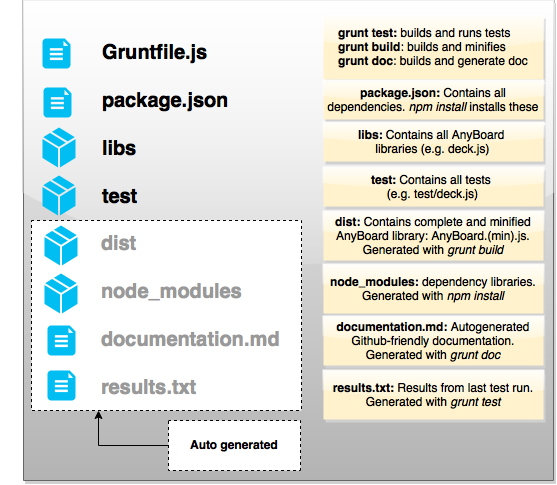
\includegraphics[width=12cm]{img/anyboard-development-overview}
\centering
\caption{Overview over the AnyBoard development files and folder structure.}
\label{fig:anyboard_development_overview}
\end{figure}

\subsection{Platform and dependency handler: NodeJS}
NodeJS\footnote{\href{http://nodejs.org}{nodejs.org}} is a platform built on Chrome's JavaScript runtime for easily building fast, scalable network applications. It is used in the project as a dependency handler and platform for our other tools, i.e. it gives us the opportunity to use the other . 

\subsubsection{Motivation}
We have chosen to use NodeJS as a tool in this project due to the active community around it, which has resulted in it being a reliable platform with a rich variety of tools that can be found and used with it. In this project, it provides us with a large set of possible tools and libraries to simplify development. It also gathers all dependencies and specifies them in one file, and provides a \emph{\textbf{simple setup}} of dependencies for the environment. 

Being the by far most dominent JavaScript-based platform and something that we have previous experience with, we have not considered other options.

\subsubsection{Usage}
In figure \ref{fig:anyboard_development_overview} \emph{package.json} is a node package file for AnyBoard. It gives meta data about AnyBoard, such as location of online repository and version number, in addition to specifying all dependencies that should be installed in order to set up the development environment. Installing all dependencies is as easy as installing NodeJS, followed by navigation to the folder in a terminal and typing \emph{npm install}.

Upon installing dependencies, those are automatically installed under the \emph{node\_modules} folder, shown in the auto generated section of figure \ref{fig:anyboard_development_overview}.

\subsubsection{Replacing NodeJS}
Not using or replacing NodeJS will require changing most of the development environment, including test framework and task runner, but has no effect on the functionality of the AnyBoard library.

\subsection{Test framework: MochaJS}
Mocha \footnote{\href{http://mochajs.org/}{mochajs.org}} is a JavaScript-based test framework. It is used in the project in providing an easy to understand syntax in writiting tests, and reports the results of tests in a readable manner (see figure \ref{fig:mocha_result}). 

\subsubsection{Motivation}
Testing frameworks provides a clear syntax for testing, as well as methods and constructs for asserting whether or not function work as intended. Using a test framework and \emph{\textbf{writing tests}} for our library provides confidence to developers that they don't break the code unknowingly when changing the code. It also \emph{\textbf{provides examples}} of how to use the library.

We have chosen MochaJS over alternatives like UnitJS\emph{\href{http://unitjs.com/}{unitjs.com}} and VowsJS due to our familiarity with it, and great reporting format.

\subsubsection{Usage}
Our tests are located within the \emph{test} library shown in figure \ref{fig:anyboard_development_overview}. They are named with the same name as the library in the \emph{libs} folder that they test. All .js files placed in this folder will automatically be run by our MochaJS installation upon running \emph{grunt test} from the console when located in this folder.

\subsubsection{Replacing MochaJS}
Changing the choice of test framework will require rewriting at least parts of the tests, but has no effect on the functionality or build of the AnyBoard library, nor documentation.

\begin{figure}[ht]
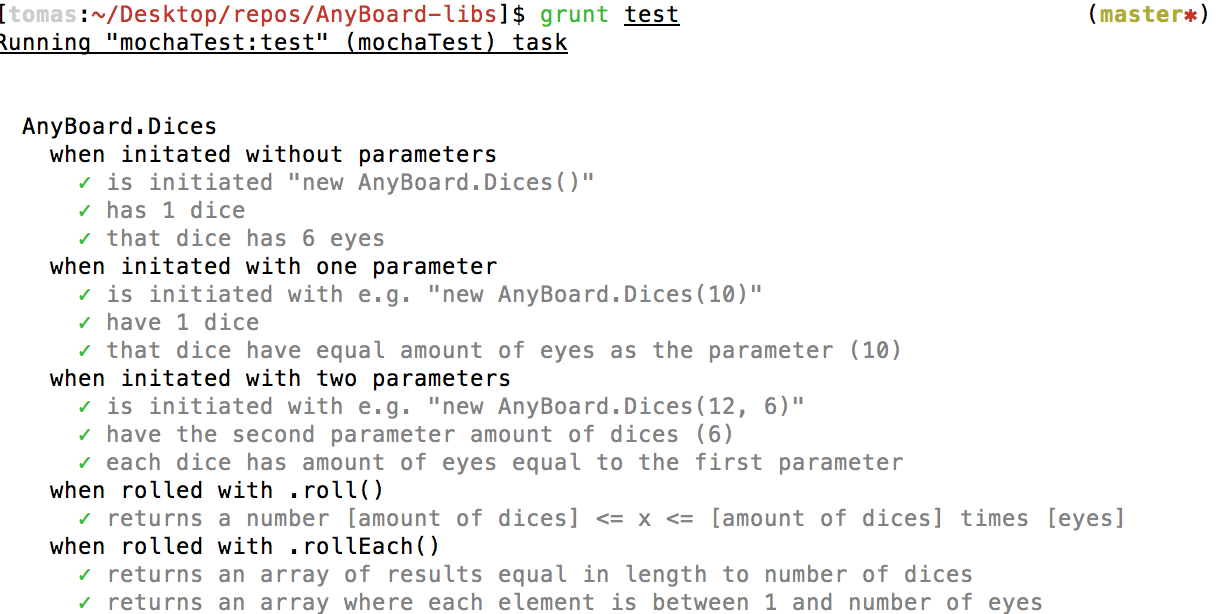
\includegraphics[width=12cm]{img/mocha-result}
\centering
\caption{Human readable test results from unit tests made with Mocha test framework.}
\label{fig:mocha_result}
\end{figure}

\subsection{Task runner: Grunt}
Grunt\footnote{\href{http://gruntjs.com/}{gruntjs.com}} is a JavaScript-based Task Runner. It is used in the project to simplify building the AnyBoard library, generating documentation and running tests.

\subsubsection{Motivation}
Task runners simplify common tasks, such as concatination of files, compilations etc. by allowing us to create shorthand commands for doing larger tasks. Our motivation is simplifying the creating of documentation files, concatination and minifying our library from smaller modules. 

Grunt was chosen over alternatives such as GulpJS\footnote{\href{http://gulpjs.com/}{gulpjs.com}} and BroccoliJS\footnote{\href{http://broccolijs.com/}{broccolijs.com}} due to our prior experience with it, as well as larger community.

\subsubsection{Usage}
\emph{Gruntfile.js} as shown on top in figure \ref{fig:anyboard_development_overview}. The file specifies 7 different tasks, that is run by \emph{grunt "taskName"}, where the different "taskName" are specified in bold below. The first four tasks are simple tasks that have names dictated by a corresponding grunt module, whereas the last three are combinded tasks of which we have selected the name.

\begin{itemize}
\item \textbf{concat} - concatinates all javascript files located in \emph{lib} folder into one file, that is then put into \emph{dist/AnyBoard.js}.
\item \textbf{uglify} - Takes \emph{dist/AnyBoard.js} and compresses/minifies it, and stores it in \emph{dist/AnyBoard.min.js}
\item \textbf{mochaTest} - runs all javascript files located in the \emph{test} folder, and report their successes to the console. The result is also (over-) written to \emph{results.txt}
\item \textbf{jsdoc2md} - reads through \emph{dist/AnyBoard.js} and interprets the commenting. A markdown-file is generated and (over-) written to \emph{documentation.md}
\item \textbf{build} - runs \emph{concat} followed by \emph{uglify}
\item \textbf{test} - runs \emph{build} followed by \emph{mochaTest}
\item \textbf{doc} - runs \emph{build} followed by \emph{jsdoc2md}
\end{itemize}

\subsubsection{Replacing Grunt}
Replacing Grunt with Gulp, Broccoli or another task runner will involve replacing grunt modules specified in \emph{package.json} with modules designed for the new task runner, as well as replacing the \emph{Gruntfile.js} file with a new configuration file. It has no effect on the functionality of the AnyBoard library.

\subsection{Documentation generation: JSDoc and grunt-jsdoc-to-markdown}
JSDoc\footnote{\href{http://usejsdoc.org/}{usejsdoc.org} - a JavaScript documentation syntax and parser} is a standardized way of documenting JavaScript code. It allows IDEs\footnote{IDE is shorthand for Integrated Development Environment and is simply put a rich featured editor.} to give assisting information to a developer about the code he's using, which classes and methods are available, what they return, take as parameters etc. 

In addition, software plugins for our development platform (NodeJS + Grunt) exist that allows us to generate automatic documentation based on JSDoc syntax.

\subsubsection{Motivation}
Documenting code usually makes the further development and maintainance of code simpler. Doing it in certain ways, will also allow developers that create games with the AnyBoard libraries to be informed of which AnyBoard classes and methods that are available in his environment, as well as providing parameter list and types, provided they use a compatible IDE.

A third reason is the automatic generation of human readable documentation files, such as HTML or MarkDown files, that can be used to inform new developers of their available tools in the AnyBoard platform. Generating this documentation automatically instead of writing it manually saves us time, and gives us \emph{\textbf{consistency between different sources of documentation}}, namely from the IDE, inline code and online documentation.

We have chosen to document our code with JSDoc-oriented syntax over YUIDoc and Doxx due to JSDoc doing source parsing\footnote{JSDoc consideres source code in addition to comments in order to generate documentation}, and high extensability. 

For the plugin that runs the documentation generation, we have used grunt-jsdoc-to-markdown\footnote{\href{https://www.npmjs.com/package/grunt-jsdoc-to-markdown}{grunt-jsdoc-to-markdown} - a grunt package generating Github friendly documentation generator of JavaScript files commented with JSDoc syntax, that we decided to use}), over jsdox\footnote{\href{https://www.npmjs.com/package/grunt-jsdox}{grunt-jsdox} - a another documentation generator of Javascript files using JSDoc syntax} due to its very readable output designed for Github pages (which the project already uses).

\begin{figure}[ht]
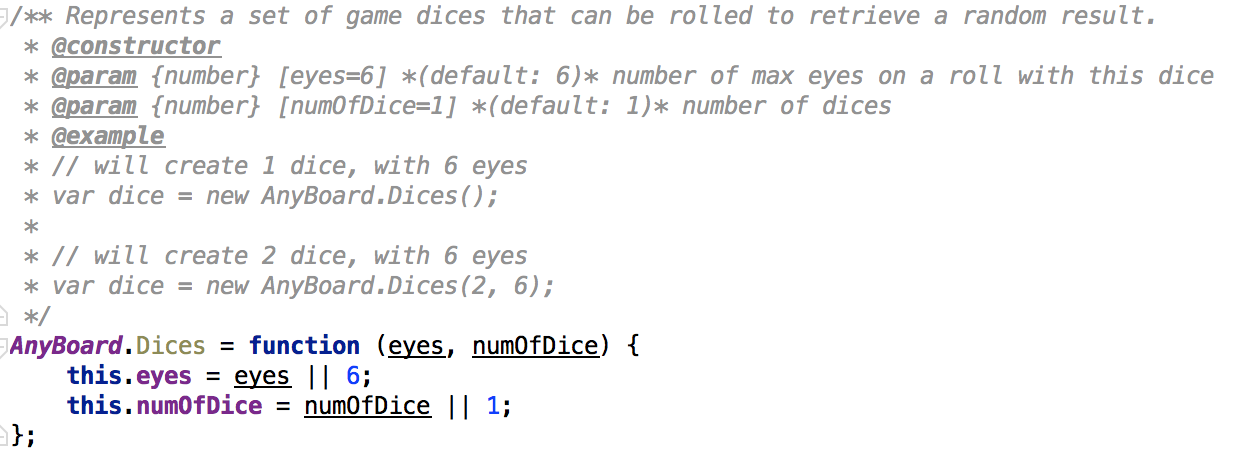
\includegraphics[width=12cm]{img/jsdoc-example}
\centering
\caption{Example of jsdoc commenting in source code.}
\label{fig:jsdoc_example}
\end{figure}

\begin{figure}[ht]
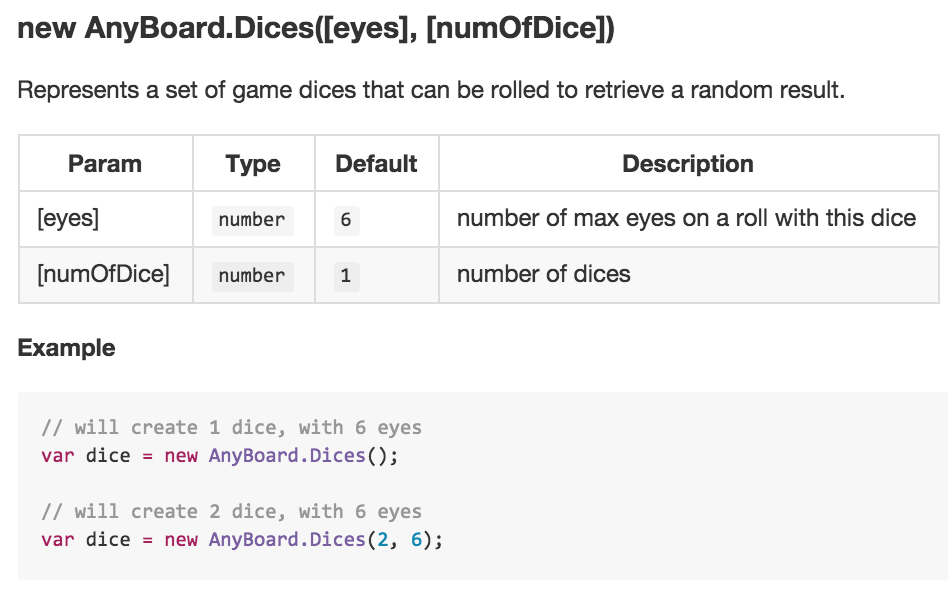
\includegraphics[width=12cm]{img/jsdoc-result}
\centering
\caption{Example of generated documentation by grunt-jsdoc-to-markdown.}
\label{fig:jsdoc_result}
\end{figure}

\subsubsection{Usage}
All source files are commented with JSDoc-syntax, see figure \ref{fig:jsdoc_example}. Most IDEs and some regular editors will automatically pick up on these comments and assist developers with writing code.

Our grunt command \emph{grunt doc}, autogenerates the \emph{documentation.md} documentation file, see \ref{fig:jsdoc_result}

\subsubsection{Replacing JSDoc}
Minor changes would be required to all source file comments in order to change to a different syntax for commenting. In addition, one would naturally have to replace grunt-jsdoc-to-markdown.

\subsubsection{Replacing grunt-jsdoc-to-markdown}
Replacing grunt-jsdoc-to-markdown will require finding a suitable grunt-compatible jsdoc compatible documentation generator, and replacing \emph{grunt-jsdoc-to-markdown} in the \emph{package.json} file.

\section{AnyBoard entities} \label{impl:entities}

\subsection{Players} 


\subsection{Decks of cards}


\subsection{Resources and transactions}

\subsection{Dice}

\subsection{Summary}


\section{Phone-Token communication} \label{impl:ble_communication}
Tokens are the physical objects for players to interact with during the game play, such as a pawns or dices. The previous work with the Don't Panic game was done using Sifteo cubes\footnote{Sifteo cubes, a commercial hardware piece that was originally used for Don't Panic \href{https://en.wikipedia.org/wiki/Sifteo\_cubes}{https://en.wikipedia.org/wiki/Sifteo\_cubes}}, a commercial device that could be adapted to work with Don't Panic using Bluetooth communication. Sifteo cubes are no longer aquireable and the lack of alternatives has led to prototyping at NTNU of a new Arduino-based token by Simone Mora. This thesis has been written with Simone as co-supervisor, and the AnyBoard framework has therefore been tested with and constructed with that token spesifically in mind, which we will from now on address as AnyBoard Pawn. 

We have also tested with a commercially available general purpose Arduino-based chip, The Lightblue Bean\footnote{The LightBlue bean (\href{http://punchthrough.com/bean/}{punchthrough.com/bean}) is a small commercially available Ardunio-based chip with built in LED, accelerometer and thermometer}.

We have two setups with LightBlue bean. One 
Both of these chips are made with Bluetooth communication as standard communication channel, and as such, AnyBoard is created with Bluetooth communication in mind.

However, we have separated out \emph{Token Drivers} as a separate part

Even though we have worked with specific hardware, namely AnyToken and The LightBlue Bean, keeping code \textbf{\emph{decoupled}} is a priority, as mentioned in section \ref{sec:requirements}. A goal [TODO: reference to systems design] is for developers to be able to a) use different tokens simulatiously and, b) easily be able to develop support for new tokens that, c) might not necessarily be communicating over bluetooth. We have chosen 

\subsection{Token drivers}
[TODO: Insert a figure explaining the loading of drivers]

\subsection{Communication protocol implementation}
The talk of Services, Characteristics and Descriptors???
How we map each of them to a capability of the token.

How it relates to our capability-mapping?

- 20 byte maximum BLE packet size. 
- Caused problems with our initial implementation of JSON protocol (worked fine over USB, of course)
- 13 byte max packet bean size due to own protocol.
- This limitation is available to overcome by implementing concatination and breaking apart packets on each end.

\subsection{Communcation}
[TODO: Insert a figure of Bluetooth communication]

[TODO: Insert a figure explaini]

\section{Implementation: Board design editor and creation}
- Planned but not executed
- Not time
How board games are made and read by the engine.

\section{Implementation: Game engine and enforcing rules}

How to create game concepts, entities and rules + How the game engine works and it implements them. 

\newpage